\documentclass{article}
\usepackage[T1]{fontenc}
\usepackage[utf8]{inputenc}
\usepackage{lmodern}
\usepackage[T1]{fontenc}
\usepackage[utf8]{inputenc}
\usepackage{lmodern}
\usepackage[T1]{fontenc}
\usepackage[utf8]{inputenc}
\usepackage{lmodern}
\usepackage[tmargin=1cm,lmargin=1cm]{geometry}
\usepackage{tikz}
\usepackage{pgfplots}
\pgfplotsset{compat=newest}
\usepackage{pgfplots}


\begin{document}
\section{Series: h}
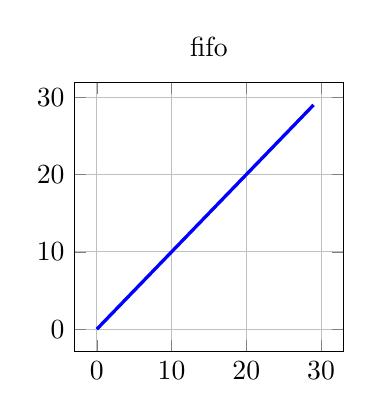
\begin{tikzpicture}
\begin{axis}[title=fifo, height=5cm, width=5cm, grid=major, xmin=({-}3.0), xmax=(33.0), ymin=({-}2.9), ymax=(31.9)]
\addplot[very thick,color=blue] coordinates {
(0,0)
(1,1)
(2,2)
(3,3)
(4,4)
(5,5)
(6,6)
(7,7)
(8,8)
(9,9)
(10,10)
(11,11)
(12,12)
(13,13)
(14,14)
(15,15)
(16,16)
(17,17)
(18,18)
(19,19)
(20,20)
(21,21)
(22,22)
(23,23)
(24,24)
(25,25)
(26,26)
(27,27)
(28,28)
(29,29)
};


\end{axis}
\end{tikzpicture}
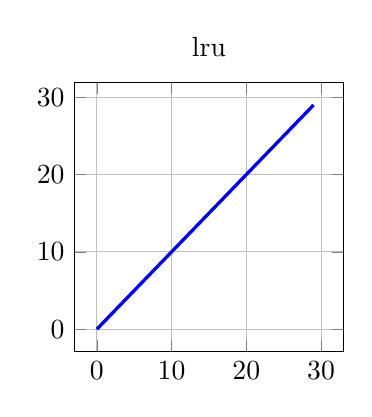
\begin{tikzpicture}
\begin{axis}[title=lru, height=5cm, width=5cm, grid=major, xmin=({-}3.0), xmax=(33.0), ymin=({-}2.9), ymax=(31.9)]
\addplot[very thick,color=blue] coordinates {
(0,0)
(1,1)
(2,2)
(3,3)
(4,4)
(5,5)
(6,6)
(7,7)
(8,8)
(9,9)
(10,10)
(11,11)
(12,12)
(13,13)
(14,14)
(15,15)
(16,16)
(17,17)
(18,18)
(19,19)
(20,20)
(21,21)
(22,22)
(23,23)
(24,24)
(25,25)
(26,26)
(27,27)
(28,28)
(29,29)
};


\end{axis}
\end{tikzpicture}
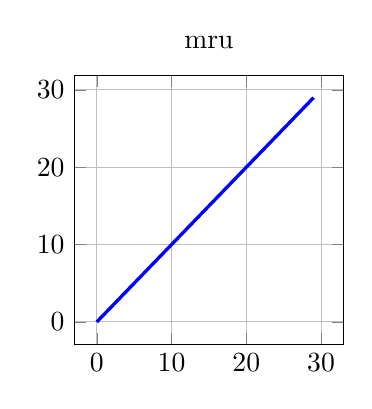
\begin{tikzpicture}
\begin{axis}[title=mru, height=5cm, width=5cm, grid=major, xmin=({-}3.0), xmax=(33.0), ymin=({-}2.9), ymax=(31.9)]
\addplot[very thick,color=blue] coordinates {
(0,0)
(1,1)
(2,2)
(3,3)
(4,4)
(5,5)
(6,6)
(7,7)
(8,8)
(9,9)
(10,10)
(11,11)
(12,12)
(13,13)
(14,14)
(15,15)
(16,16)
(17,17)
(18,18)
(19,19)
(20,20)
(21,21)
(22,22)
(23,23)
(24,24)
(25,25)
(26,26)
(27,27)
(28,28)
(29,29)
};


\end{axis}
\end{tikzpicture}
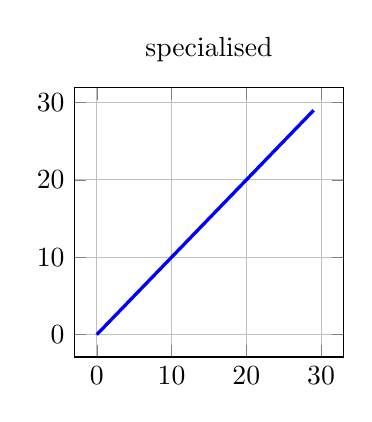
\begin{tikzpicture}
\begin{axis}[title=specialised, height=5cm, width=5cm, grid=major, xmin=({-}3.0), xmax=(33.0), ymin=({-}2.9), ymax=(31.9)]
\addplot[very thick,color=blue] coordinates {
(0,0)
(1,1)
(2,2)
(3,3)
(4,4)
(5,5)
(6,6)
(7,7)
(8,8)
(9,9)
(10,10)
(11,11)
(12,12)
(13,13)
(14,14)
(15,15)
(16,16)
(17,17)
(18,18)
(19,19)
(20,20)
(21,21)
(22,22)
(23,23)
(24,24)
(25,25)
(26,26)
(27,27)
(28,28)
(29,29)
};


\end{axis}
\end{tikzpicture}


\section{Series: math.log10(h / h + ncm + cm)}
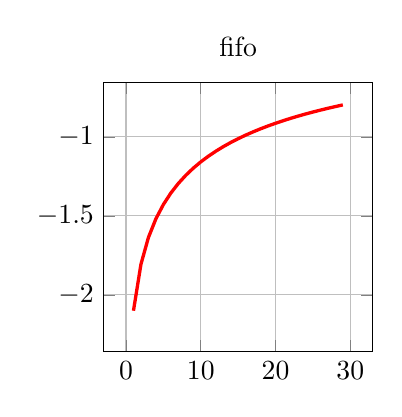
\begin{tikzpicture}
\begin{axis}[title=fifo, height=5cm, width=5cm, grid=major, xmin=({-}3.0), xmax=(33.0), ymin=({-}2.3595), ymax=({-}0.6557)]
\addplot[very thick,color=red] coordinates {
(1,-2.100370545117563)
(2,-1.806179973983887)
(3,-1.6368220975871743)
(4,-1.5185139398778875)
(5,-1.428134794028789)
(6,-1.3553876579865738)
(7,-1.2947810463869796)
(8,-1.2430380486862944)
(9,-1.1980458349437315)
(10,-1.1583624920952496)
(11,-1.122960170626212)
(12,-1.0910804693473326)
(13,-1.0621479067488444)
(14,-1.0357155522665344)
(15,-1.0114294617807817)
(16,-0.9890046156985368)
(17,-0.9682081655761486)
(18,-0.9488474775526187)
(19,-0.930761413589802)
(20,-0.9138138523837167)
(21,-0.8978887933061359)
(22,-0.8828866009036566)
(23,-0.868721085360681)
(24,-0.8553172051959429)
(25,-0.8426092396105621)
(26,-0.8305393198433318)
(27,-0.8190562381499067)
(28,-0.8081144737610868)
(29,-0.7976733900861187)
};


\end{axis}
\end{tikzpicture}
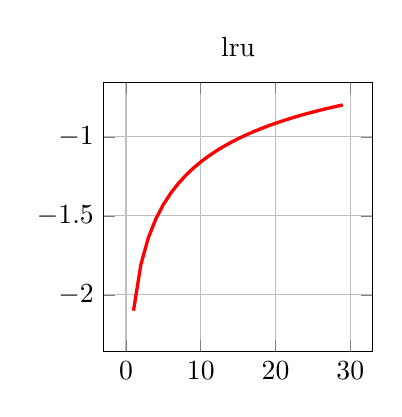
\begin{tikzpicture}
\begin{axis}[title=lru, height=5cm, width=5cm, grid=major, xmin=({-}3.0), xmax=(33.0), ymin=({-}2.3595), ymax=({-}0.6557)]
\addplot[very thick,color=red] coordinates {
(1,-2.100370545117563)
(2,-1.806179973983887)
(3,-1.6368220975871743)
(4,-1.5185139398778875)
(5,-1.428134794028789)
(6,-1.3553876579865738)
(7,-1.2947810463869796)
(8,-1.2430380486862944)
(9,-1.1980458349437315)
(10,-1.1583624920952496)
(11,-1.122960170626212)
(12,-1.0910804693473326)
(13,-1.0621479067488444)
(14,-1.0357155522665344)
(15,-1.0114294617807817)
(16,-0.9890046156985368)
(17,-0.9682081655761486)
(18,-0.9488474775526187)
(19,-0.930761413589802)
(20,-0.9138138523837167)
(21,-0.8978887933061359)
(22,-0.8828866009036566)
(23,-0.868721085360681)
(24,-0.8553172051959429)
(25,-0.8426092396105621)
(26,-0.8305393198433318)
(27,-0.8190562381499067)
(28,-0.8081144737610868)
(29,-0.7976733900861187)
};


\end{axis}
\end{tikzpicture}
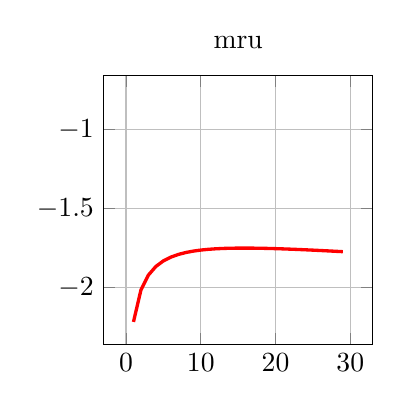
\begin{tikzpicture}
\begin{axis}[title=mru, height=5cm, width=5cm, grid=major, xmin=({-}3.0), xmax=(33.0), ymin=({-}2.3595), ymax=({-}0.6557)]
\addplot[very thick,color=red] coordinates {
(1,-2.2174839442139063)
(2,-2.0149403497929366)
(3,-1.9208187539523751)
(4,-1.866287339084195)
(5,-1.8312296938670634)
(6,-1.807309479124857)
(7,-1.7903857068006552)
(8,-1.7781512503836436)
(9,-1.769213162595861)
(10,-1.7626785637274363)
(11,-1.7579478642953565)
(12,-1.7546031286088541)
(13,-1.752343986777358)
(14,-1.7509489675311822)
(15,-1.7502511875699738)
(16,-1.7501225267834002)
(17,-1.7504630163985695)
(18,-1.7511935371459255)
(19,-1.7522506804107079)
(20,-1.7535830588929067)
(21,-1.7551486105502372)
(22,-1.7569125968637516)
(23,-1.758846095188257)
(24,-1.760924848409133)
(25,-1.763128376799137)
(26,-1.7654392848675058)
(27,-1.7678427150026705)
(28,-1.770325912871687)
(29,-1.7728778787880963)
};


\end{axis}
\end{tikzpicture}
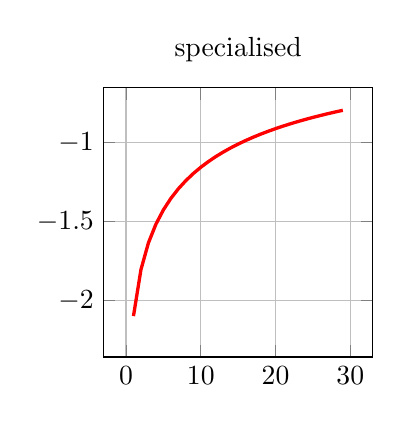
\begin{tikzpicture}
\begin{axis}[title=specialised, height=5cm, width=5cm, grid=major, xmin=({-}3.0), xmax=(33.0), ymin=({-}2.3595), ymax=({-}0.6557)]
\addplot[very thick,color=red] coordinates {
(1,-2.100370545117563)
(2,-1.806179973983887)
(3,-1.6368220975871743)
(4,-1.5185139398778875)
(5,-1.428134794028789)
(6,-1.3553876579865738)
(7,-1.2947810463869796)
(8,-1.2430380486862944)
(9,-1.1980458349437315)
(10,-1.1583624920952496)
(11,-1.122960170626212)
(12,-1.0910804693473326)
(13,-1.0621479067488444)
(14,-1.0357155522665344)
(15,-1.0114294617807817)
(16,-0.9890046156985368)
(17,-0.9682081655761486)
(18,-0.9488474775526187)
(19,-0.930761413589802)
(20,-0.9138138523837167)
(21,-0.8978887933061359)
(22,-0.8828866009036566)
(23,-0.868721085360681)
(24,-0.8553172051959429)
(25,-0.8426092396105621)
(26,-0.8305393198433318)
(27,-0.8190562381499067)
(28,-0.8081144737610868)
(29,-0.7976733900861187)
};


\end{axis}
\end{tikzpicture}


\section{Series: math.log10(h / h + ncm)}
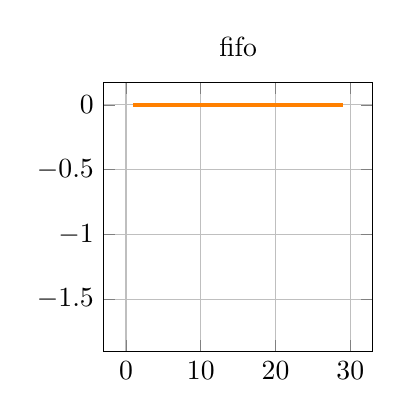
\begin{tikzpicture}
\begin{axis}[title=fifo, height=5cm, width=5cm, grid=major, xmin=({-}3.0), xmax=(33.0), ymin=({-}1.9056), ymax=(0.1732)]
\addplot[very thick,color=orange] coordinates {
(1,0.0)
(2,0.0)
(3,0.0)
(4,0.0)
(5,0.0)
(6,0.0)
(7,0.0)
(8,0.0)
(9,0.0)
(10,0.0)
(11,0.0)
(12,0.0)
(13,0.0)
(14,0.0)
(15,0.0)
(16,0.0)
(17,0.0)
(18,0.0)
(19,0.0)
(20,0.0)
(21,0.0)
(22,0.0)
(23,0.0)
(24,0.0)
(25,0.0)
(26,0.0)
(27,0.0)
(28,0.0)
(29,0.0)
};


\end{axis}
\end{tikzpicture}
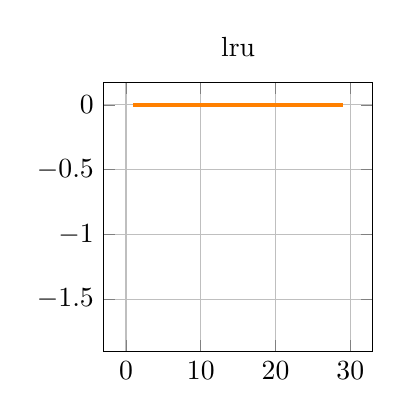
\begin{tikzpicture}
\begin{axis}[title=lru, height=5cm, width=5cm, grid=major, xmin=({-}3.0), xmax=(33.0), ymin=({-}1.9056), ymax=(0.1732)]
\addplot[very thick,color=orange] coordinates {
(1,0.0)
(2,0.0)
(3,0.0)
(4,0.0)
(5,0.0)
(6,0.0)
(7,0.0)
(8,0.0)
(9,0.0)
(10,0.0)
(11,0.0)
(12,0.0)
(13,0.0)
(14,0.0)
(15,0.0)
(16,0.0)
(17,0.0)
(18,0.0)
(19,0.0)
(20,0.0)
(21,0.0)
(22,0.0)
(23,0.0)
(24,0.0)
(25,0.0)
(26,0.0)
(27,0.0)
(28,0.0)
(29,0.0)
};


\end{axis}
\end{tikzpicture}
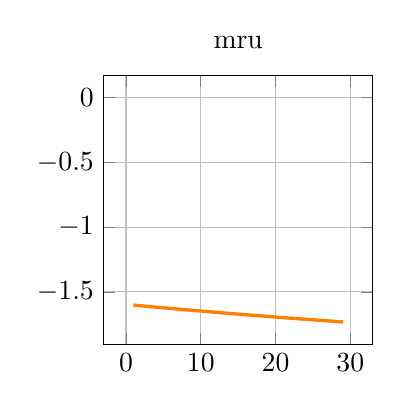
\begin{tikzpicture}
\begin{axis}[title=mru, height=5cm, width=5cm, grid=major, xmin=({-}3.0), xmax=(33.0), ymin=({-}1.9056), ymax=(0.1732)]
\addplot[very thick,color=orange] coordinates {
(1,-1.6020599913279623)
(2,-1.6074550232146685)
(3,-1.6127838567197355)
(4,-1.6180480967120927)
(5,-1.6232492903979006)
(6,-1.6283889300503116)
(7,-1.6334684555795866)
(8,-1.6384892569546374)
(9,-1.6434526764861874)
(10,-1.6483600109809315)
(11,-1.6532125137753437)
(12,-1.6580113966571124)
(13,-1.662757831681574)
(14,-1.667452952889954)
(15,-1.6720978579357175)
(16,-1.6766936096248666)
(17,-1.6812412373755872)
(18,-1.6857417386022637)
(19,-1.6901960800285136)
(20,-1.6946051989335686)
(21,-1.6989700043360187)
(22,-1.7032913781186614)
(23,-1.7075701760979363)
(24,-1.711807229041191)
(25,-1.7160033436347992)
(26,-1.7201593034059568)
(27,-1.7242758696007892)
(28,-1.7283537820212285)
(29,-1.7323937598229686)
};


\end{axis}
\end{tikzpicture}
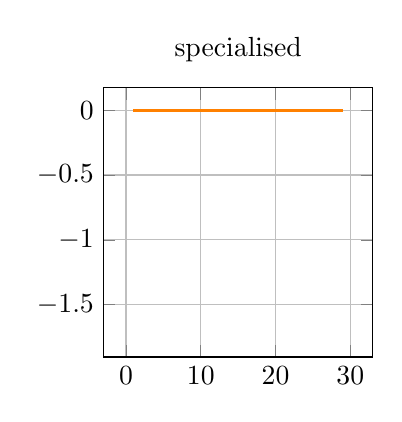
\begin{tikzpicture}
\begin{axis}[title=specialised, height=5cm, width=5cm, grid=major, xmin=({-}3.0), xmax=(33.0), ymin=({-}1.9056), ymax=(0.1732)]
\addplot[very thick,color=orange] coordinates {
(1,0.0)
(2,0.0)
(3,0.0)
(4,0.0)
(5,0.0)
(6,0.0)
(7,0.0)
(8,0.0)
(9,0.0)
(10,0.0)
(11,0.0)
(12,0.0)
(13,0.0)
(14,0.0)
(15,0.0)
(16,0.0)
(17,0.0)
(18,0.0)
(19,0.0)
(20,0.0)
(21,0.0)
(22,0.0)
(23,0.0)
(24,0.0)
(25,0.0)
(26,0.0)
(27,0.0)
(28,0.0)
(29,0.0)
};


\end{axis}
\end{tikzpicture}


\end{document}